\documentclass{article}
\usepackage[T1]{fontenc}
\usepackage[utf8]{inputenc}
\usepackage{lmodern}
\usepackage[margin=0.75in]{geometry}
\usepackage{subcaption}
\usepackage{xcolor}
\usepackage{needspace}
\usepackage{graphicx}
\usepackage{subcaption}


\begin{document}
\makeatletter
\setlength{\@fptop}{0pt}
\makeatother
\renewcommand{\baselinestretch}{1.0}
\begin{center}
\Large{\textbf{Sample Quality Results}}
\end{center}
\section{Basic Statistics}
\begin{description}
\item[Sample:]
04{-}D15{-}22373{-}HT{-}Nextera{-}Myeloid{-}Val1{-}Repeat\_S4\_L001
\item[File type:]
Conventional base calls
\item[Encoding:]
Sanger / Illumina 1.9
\end{description}
\begin{tabular}{p{5.5cm}|c|c|c|c}
&R1&&R2&\\
\hline
&Before trimming&After trimming&Before trimming&After trimming\\
\hline
Total Sequences&616751&310338&616751&310338\\
Sequences flagged as poor quality&0&0&0&0\\
Sequence length&151&50{-}150&151&50{-}150\\
\%GC&43&40&43&40\\
\end{tabular}


\section{FastQC}


\begin{figure}[!htb]
\caption{Per base sequence quality}
\centering
\begin{subfigure}{0.45\linewidth}
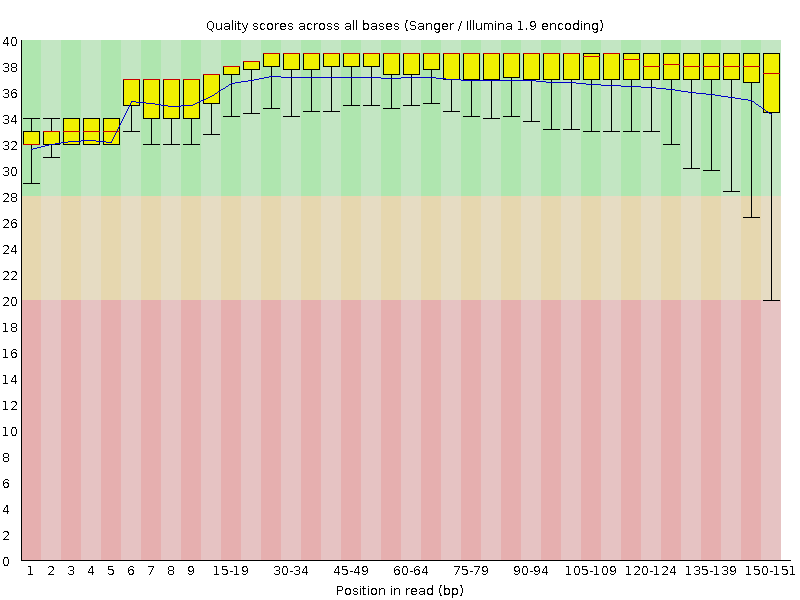
\includegraphics[width=\linewidth]{04-D15-22373-HT-Nextera-Myeloid-Val1-Repeat_S4_L001_R1_001_fastqc/Images/per_base_quality.png}
\caption{R1 BEFORE trimming}
\end{subfigure}
\begin{subfigure}{0.45\linewidth}
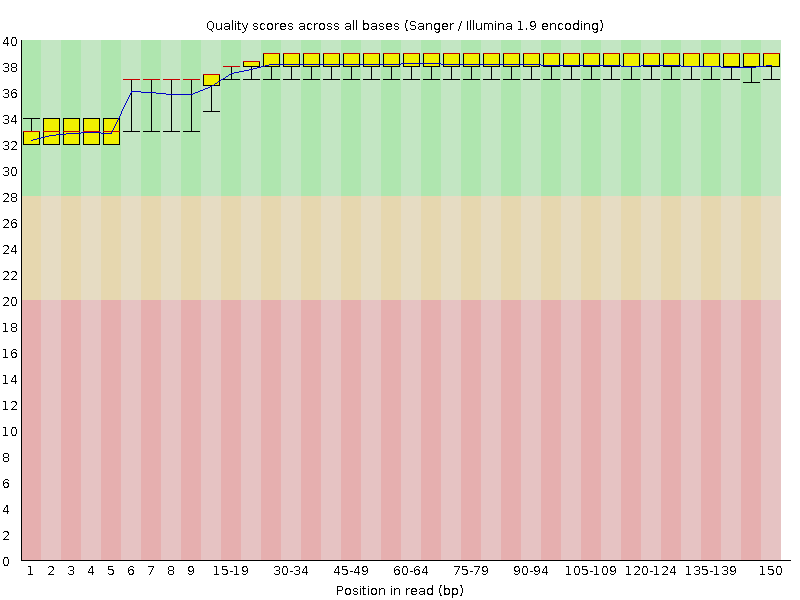
\includegraphics[width=\linewidth]{04-D15-22373-HT-Nextera-Myeloid-Val1-Repeat_S4_L001_R1_001.qfilter_fastqc/Images/per_base_quality.png}
\caption{R1 AFTER trimming \textcolor{green}{PASS}}
\end{subfigure}
\begin{subfigure}{0.45\linewidth}
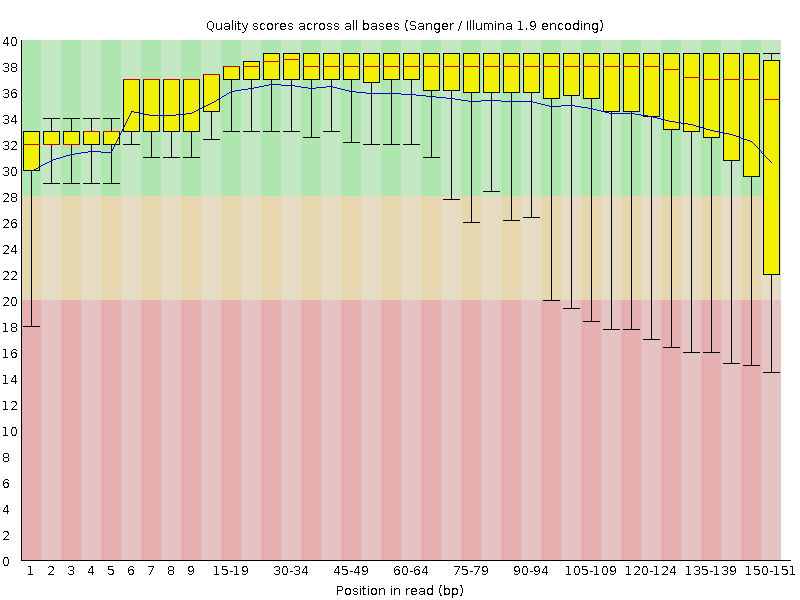
\includegraphics[width=\linewidth]{04-D15-22373-HT-Nextera-Myeloid-Val1-Repeat_S4_L001_R2_001_fastqc/Images/per_base_quality.png}
\caption{R2 BEFORE trimming}
\end{subfigure}
\begin{subfigure}{0.45\linewidth}
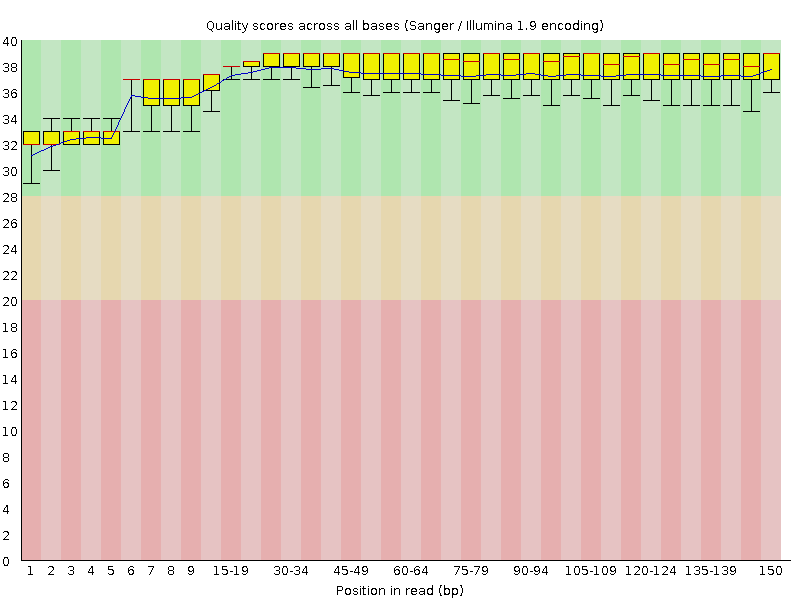
\includegraphics[width=\linewidth]{04-D15-22373-HT-Nextera-Myeloid-Val1-Repeat_S4_L001_R2_001.qfilter_fastqc/Images/per_base_quality.png}
\caption{R2 AFTER trimming \textcolor{green}{PASS}}
\end{subfigure}
\end{figure}




\begin{figure}[!htb]
\caption{Per sequence GC content}
\centering
\begin{subfigure}{0.45\linewidth}
\vspace{5 mm}
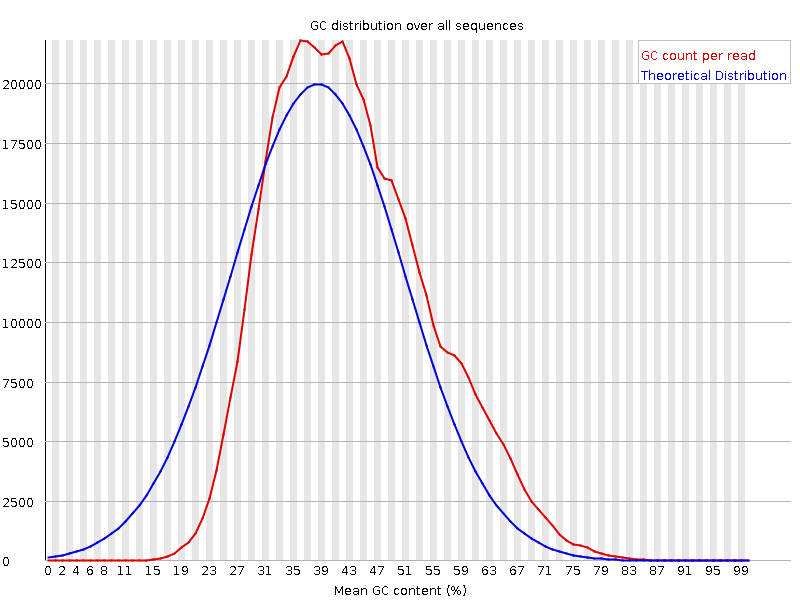
\includegraphics[width=\linewidth]{04-D15-22373-HT-Nextera-Myeloid-Val1-Repeat_S4_L001_R1_001_fastqc/Images/per_sequence_gc_content.png}
\caption{R1 BEFORE trimming}
\end{subfigure}
\begin{subfigure}{0.45\linewidth}
\vspace{5 mm}
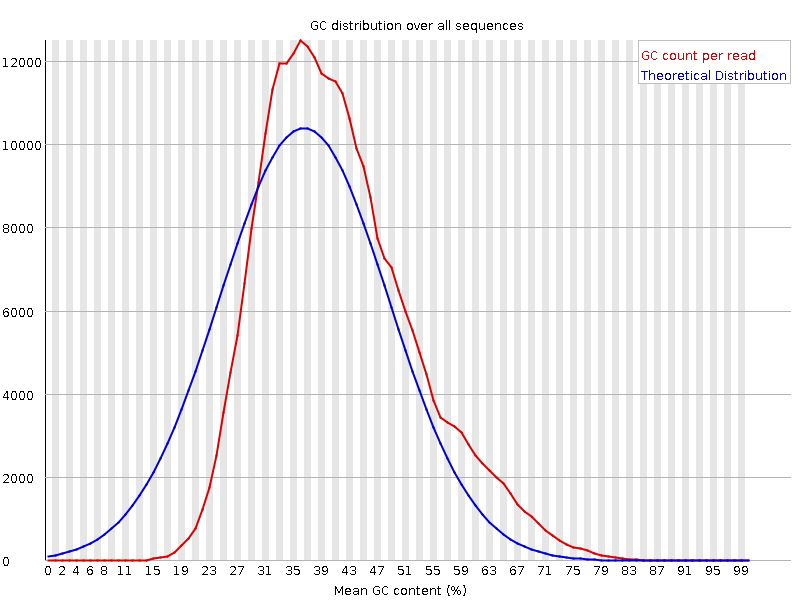
\includegraphics[width=\linewidth]{04-D15-22373-HT-Nextera-Myeloid-Val1-Repeat_S4_L001_R1_001.qfilter_fastqc/Images/per_sequence_gc_content.png}
\caption{R1 AFTER trimming \textcolor{red}{FAIL}}
\end{subfigure}
\begin{subfigure}{0.45\linewidth}
\vspace{5 mm}
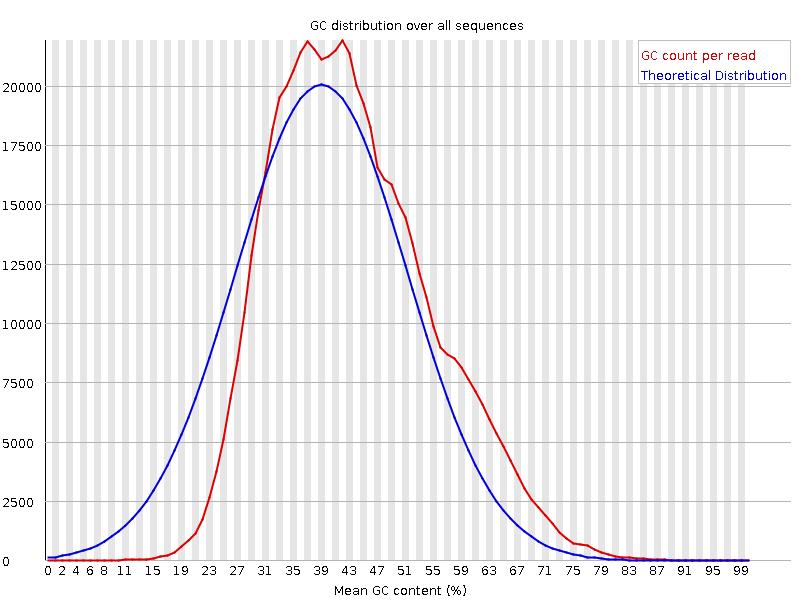
\includegraphics[width=\linewidth]{04-D15-22373-HT-Nextera-Myeloid-Val1-Repeat_S4_L001_R2_001_fastqc/Images/per_sequence_gc_content.png}
\caption{R2 BEFORE trimming}
\end{subfigure}
\begin{subfigure}{0.45\linewidth}
\vspace{5 mm}
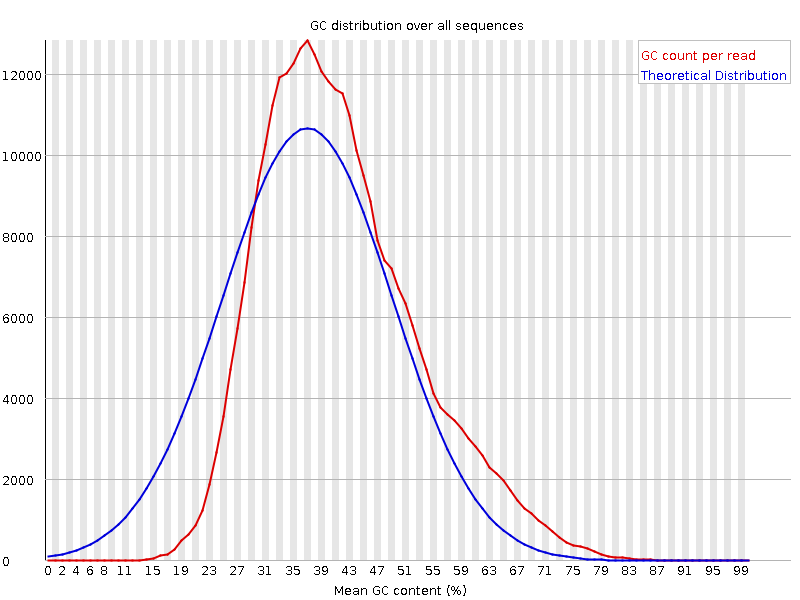
\includegraphics[width=\linewidth]{04-D15-22373-HT-Nextera-Myeloid-Val1-Repeat_S4_L001_R2_001.qfilter_fastqc/Images/per_sequence_gc_content.png}
\caption{R2 AFTER trimming \textcolor{red}{FAIL}}
\end{subfigure}
\end{figure}




\begin{figure}[!htb]
\caption{Sequence Length Distribution}
\centering
\begin{subfigure}{0.45\linewidth}
\includegraphics[width=\linewidth]{04-D15-22373-HT-Nextera-Myeloid-Val1-Repeat_S4_L001_R1_001_fastqc/Images/sequence_length_distribution.png}
\caption{R1 BEFORE trimming}
\end{subfigure}
\begin{subfigure}{0.45\linewidth}
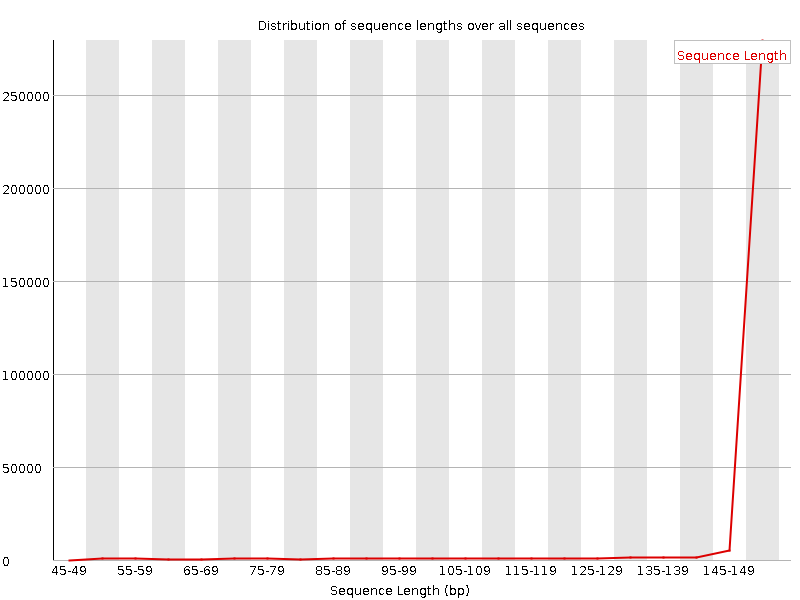
\includegraphics[width=\linewidth]{04-D15-22373-HT-Nextera-Myeloid-Val1-Repeat_S4_L001_R1_001.qfilter_fastqc/Images/sequence_length_distribution.png}
\caption{R1 AFTER trimming \textcolor{orange}{WARN}}
\end{subfigure}
\begin{subfigure}{0.45\linewidth}
\includegraphics[width=\linewidth]{04-D15-22373-HT-Nextera-Myeloid-Val1-Repeat_S4_L001_R2_001_fastqc/Images/sequence_length_distribution.png}
\caption{R2 BEFORE trimming}
\end{subfigure}
\begin{subfigure}{0.45\linewidth}
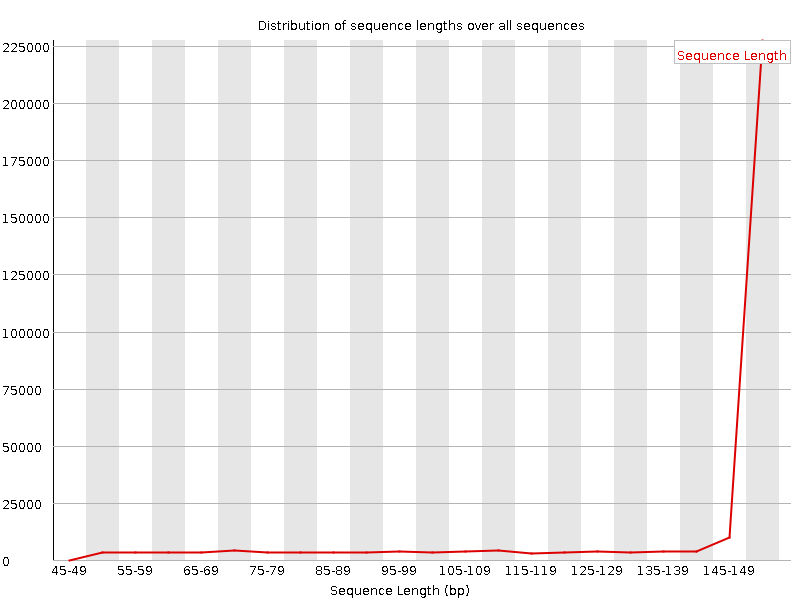
\includegraphics[width=\linewidth]{04-D15-22373-HT-Nextera-Myeloid-Val1-Repeat_S4_L001_R2_001.qfilter_fastqc/Images/sequence_length_distribution.png}
\caption{R2 AFTER trimming \textcolor{orange}{WARN}}
\end{subfigure}
\end{figure}




\begin{figure}[!htb]
\caption{Adapter Content}
\centering
\begin{subfigure}{0.45\linewidth}
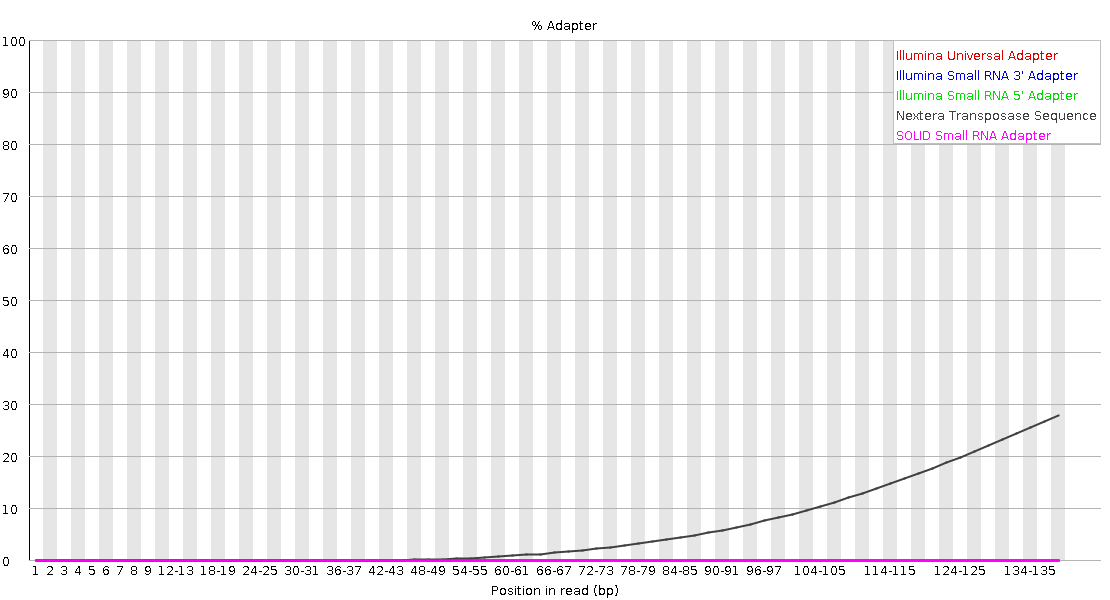
\includegraphics[width=\linewidth]{04-D15-22373-HT-Nextera-Myeloid-Val1-Repeat_S4_L001_R1_001_fastqc/Images/adapter_content.png}
\caption{R1 BEFORE trimming}
\end{subfigure}
\begin{subfigure}{0.45\linewidth}
\includegraphics[width=\linewidth]{04-D15-22373-HT-Nextera-Myeloid-Val1-Repeat_S4_L001_R1_001.qfilter_fastqc/Images/adapter_content.png}
\caption{R1 AFTER trimming \textcolor{green}{PASS}}
\end{subfigure}
\begin{subfigure}{0.45\linewidth}
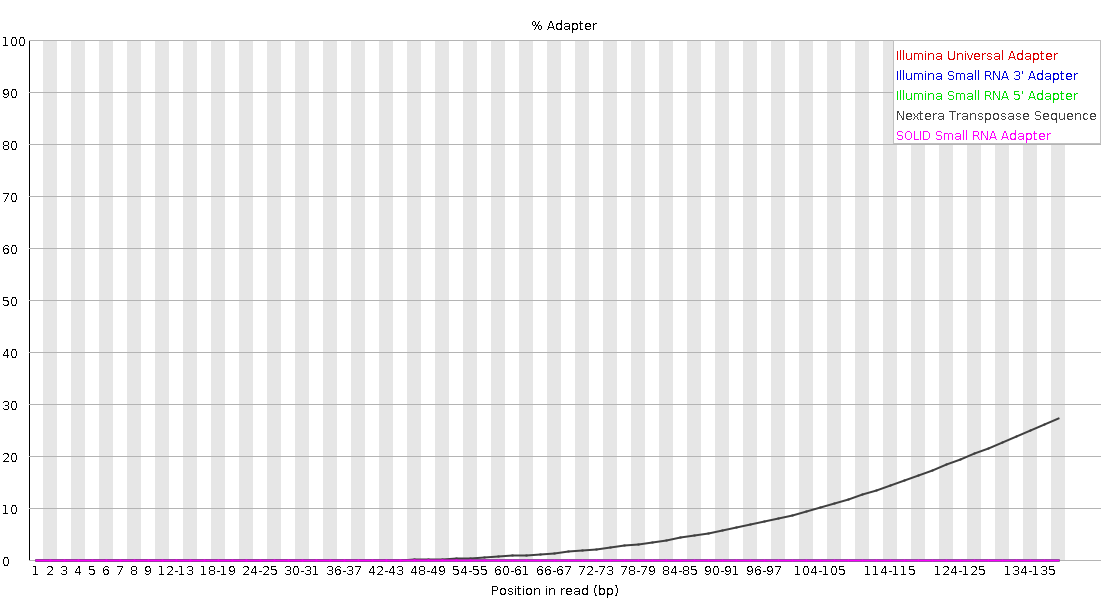
\includegraphics[width=\linewidth]{04-D15-22373-HT-Nextera-Myeloid-Val1-Repeat_S4_L001_R2_001_fastqc/Images/adapter_content.png}
\caption{R2 BEFORE trimming}
\end{subfigure}
\begin{subfigure}{0.45\linewidth}
\includegraphics[width=\linewidth]{04-D15-22373-HT-Nextera-Myeloid-Val1-Repeat_S4_L001_R2_001.qfilter_fastqc/Images/adapter_content.png}
\caption{R2 AFTER trimming \textcolor{green}{PASS}}
\end{subfigure}
\end{figure}


\needspace{1635em}
\section{BamStats}


\begin{figure}[htbp]
\centering
\begin{subfigure}{0.45\linewidth}
\includegraphics[width=\linewidth]{{04-D15-22373-HT-Nextera-Myeloid-Val1-Repeat_S4_L001_.bwa.drm.sorted.bam.stats-quals-hm}.png}
\caption{Base quality per cycle}
\end{subfigure}
\begin{subfigure}{0.45\linewidth}
\hspace{10 mm}
\includegraphics[width=\linewidth]{{04-D15-22373-HT-Nextera-Myeloid-Val1-Repeat_S4_L001_.bwa.drm.sorted.bam.stats-insert-size}.png}
\caption{Fragment size}
\end{subfigure}
\begin{subfigure}{0.45\linewidth}
\vspace{10 mm}
\includegraphics[width=\linewidth]{{04-D15-22373-HT-Nextera-Myeloid-Val1-Repeat_S4_L001_.bwa.drm.sorted.bam.stats-quals2}.png}
\caption{Quality per cycle}
\end{subfigure}
\end{figure}


\end{document}